\documentclass[a4paper, 12pt]{article}
\usepackage{geometry}
\geometry{a4paper,
            total={170mm,257mm},left=2cm,right=2cm,
            top=2cm,bottom=2cm
        }

\usepackage{mathtext}
\usepackage{amsmath}
\usepackage[T2A]{fontenc}
\usepackage[utf8]{inputenc}
\usepackage[english,russian]{babel}
\usepackage{graphicx, float}
\usepackage{tabularx, colortbl}
\usepackage{caption}
\captionsetup{labelsep=period}

\newcommand{\parag}[1]{\paragraph*{#1:}}
\DeclareSymbolFont{T2Aletters}{T2A}{cmr}{m}{it}
\newcounter{Points}
\setcounter{Points}{1}
\newcommand{\point}{\arabic{Points}. \addtocounter{Points}{1}}
\newcolumntype{C}{>{\centering\arraybackslash}X}

\author{Калинин Даниил, Б01-108}
\date{\today}
\title{Лабораторная работа 5.8.1.}

\begin{document}
\maketitle
\parindent=0cm

\parag {Цель работы}
при помощи модели абсолютно чёрного тела (АЧТ) проводятся измерения температуры, исследуется излучение накалённых тел, определяются постоянные Планка и Стефана-Больцмана. 


\parag {В работе используются}
оптический пирометр с исчезающей нитью и термопарой, накалённые тела с различной испускательной способностью.


\parag {Теоритическая справка} ~\\
Для измерения температуры тел, удалённых от наблюдателя, применяют методы оптических пирометрии, основанные на использовании зависимости испускательной способности исследуемого тела от температуры. Различают три температуры, функционально связанные с истинной термодинамической температурой и излучательной способностью тела: радиационную $T_{рад}$, цветовую $T_{цв}$ и яркостную $T_{ярк}$.

Радиационная (энергетическая) температура --- температура АЧТ, при которой его интегральная испускательная способность одинакова с интегральной испускательной способностью исследуемого тела.

Цветовая температура --- температура АЧТ, при которой отношение их спектральных испускательных способностей для двух заданных длин волн одинаково.

Яркостная температура --- температура АЧТ, при которой его спектральная испускательная способность равна спектральной испукательной способности исследуемого тела при той же длине волны. Именно эту температуру мы и будем измерять. Для вольфрама функциональная зависимость термодинамической температуры от яркостной представлена на рис. \ref{fig:wolfram}.

\begin{figure}[H]
    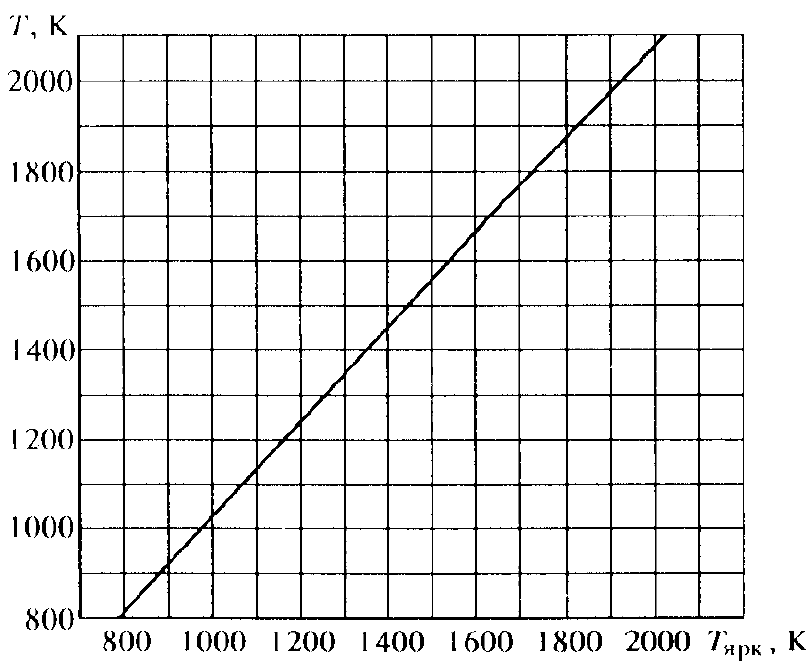
\includegraphics[scale = 0.4]{wolfram_brightness}
    \centering
    \caption{$T = f(T_{ярк})$ для вольфрама}
    \label{fig:wolfram}
\end{figure}

Закон Киргофа для излучения любого тела:

\begin{equation}
    r_{\lambda} = a_{\lambda} r_{\lambda}^{АЧТ}
\end{equation}

Для абсолютно серого тела (АСТ):

\begin{equation}
    a_{\lambda} \equiv a = const
\end{equation}

Если бы нить излучала как АЧТ, то баланс потребляемой и излучаемой энергии определялся бы соотношением:

\begin{equation}
    W = \sigma S (T^4 - T_0^4)
\end{equation}

где $W$ --- потребляемой нитью электрическая мощность, $S$ --- площадь излучаемой поверхности нити, $T$ --- температура нити, $T_0$ --- температура окружающей среды, $\sigma = 5.67 \cdot 10^{-12} ~ \dfrac{Вт}{см^2 \cdot К^4}$ --- постоянная Стефана-Больцмана.

Если считать нить серым телом и его излучение ослаблено на $\varepsilon_T$ по сравнению с АЧТ, то:

\begin{equation} \label{eq:s-b}
    W = \varepsilon_T S \sigma T^4
\end{equation}

Коэффициент $\varepsilon_T$ зависит от температуры следующим образом для вольфрама:

\begin{table}[H]
    \centering
    \begin{tabular}{|c|c|c|c|c|}
        \hline
        $T$, К  &   1700 &  1800 &  1900 &  2000 \\ \hline
        $\varepsilon_T$ & 0.209 & 0.223 & 0.236 & 0.249 \\ \hline
    \end{tabular}
    \caption {$\varepsilon_T (T)$ для вольфрама}
    \label{tab:epsT}
\end{table}

При выполнении работы также потребуется вычислить постоянную планка $h$ с помощью постоянной Стефана-Больцмана $\sigma$. Приведём необходимую формулу ниже:

\begin{equation} \label{eq:h-sigma}
    h = \sqrt[3]{\frac{2 \pi^5 k_Б^4}{15 c^2 \sigma}}
\end{equation}

\parag {Экспериментальная установка}~\\
На рис. \ref{pic:work} изображена экспериментальная установка. Она состоит из оптического пирометра 9, модели АЧТ, трёх образцов (18, 19, 20), блока питания (1) и цифровых вольтметров В7-22А и В7-38.

\begin{figure}[H]
    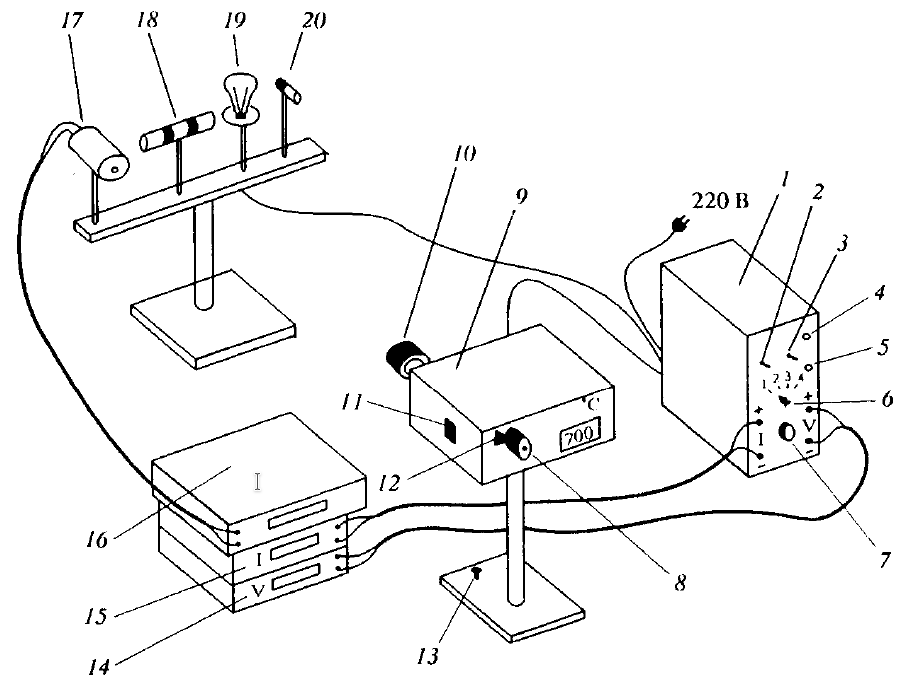
\includegraphics[scale = 0.4]{setup}
    \centering
    \caption{Схема экспериментальной установки.}
    \label{pic:work}
\end{figure}

На рисунке отмечены следующие части установки:

\begin{enumerate}
    \item Блок питания
    \item Тумблер включения питания пирометра и образцов
    \item Тумблер нагрева нити пирометра <<Быстро>> --- вверх, <<Медленно>> --- вниз
    \item Кнопка <<Нагрев нити>>
    \item Кнопка <<Охлаждение нити>>
    \item Тумблер переключения образцов
    \item Регулятор мощности нагрева образцов
    \item Окуляр пирометра
    \item Корпус пирометра
    \item Объектив пирометра
    \item Переключение диапазонов: $700-1200 ~^\circ C$ --- вниз, $1200-2000 ~^\circ C$ --- вверх
    \item Ручка перемещения красного светофильтра
    \item Регулировочный винт
    \item Вольтметр (напряжение на лампе накаливания)
    \item Амперметр (ток через образцы)
    \item Вольтметр в цепи термопары
    \item Модель АЧТ
    \item Трубка с кольцами из материалов с разной излучательной способностью
    \item Лампа накаливания
    \item Неоновая лампочка
\end{enumerate}



\parag {Ход работы} ~\\
\point Включим модель АЧТ. Далее включим пирометр и измерим температуру. Также укажем ожидаемую температуру (используя постоянную термопары $41$ мкВ). Результат занесем в таблицу \ref{tab:black_body}.

\begin{table}[H]
    \centering
    \begin{tabular}{|c|c|c|c|c|}
        \hline
        $T_{терм}$ & $T_{ярк}$ & U, мв. & Отличие, \% & направление \\ \hline
        962	&  963	& 36.82	& 0.1	 & вверх	 \\ \hline
        968	&  973	& 39.03	& 0.5	 & вниз 	 \\ \hline
        969	&  989	& 39.09	& 2.0	 & вверх	 \\ \hline
        973	&  997	& 39.14	& 2.4	 & вниз 	 \\ \hline
        974	& 1008	& 39.16	& 3.4	 & вверх	 \\ \hline
        977	& 1010	& 39.27	& 3.3	 & вниз 	 \\ \hline
        978	&  993	& 39.31	& 1.5	 & вверх	 \\ \hline
        979	& 1007	& 39.38	& 2.8	 & вниз 	 \\ \hline
        970	& 1004	& 39.04	& 3.4	 & вверх	 \\ \hline
        965	& 1001	& 38.76	& 3.6	 & вниз 	 \\ \hline
    \end{tabular}
    \caption {Измерения на АЧТ}
    \label{tab:black_body}
\end{table}

Из таблицы видно, что температуры отличаются в пределах $5\%$, т.е. пирометр настроен верно. 

\point Проверим закон Стефана-Больцмана. Для этого измерим напряжение и силу тока через лампочу с нитью накаливания прощадью $S = 0.36 ~ см^2$, изменяя её яркостную температуру от $900$ до $1900 ~^\circ C$. Результаты представлены в таблице \ref{tab:lamp}.

\begin{table}[H]
    \centering
    \begin{tabular}{|c|c|c|}
        \hline
        $T_{ярк}, ~^\circ C$ & $U$, В. & $I$, А. \\ \hline
        900	    & 1.48	 & 0.449 \\ \hline
        1000	 & 1.86	 & 0.495 \\ \hline
        1100	 & 2.35	 & 0.550 \\ \hline
        1200	 & 2.94	 & 0.611 \\ \hline
        1300	 & 3.11	 & 0.628 \\ \hline
        1400	 & 3.78	 & 0.692 \\ \hline
        1500	 & 5.01	 & 0.800 \\ \hline
        1600	 & 5.87	 & 0.869 \\ \hline
        1700	 & 7.61	 & 0.998 \\ \hline
        1800	 & 7.82	 & 1.011 \\ \hline
        1900	 & 8.12	 & 1.031 \\ \hline
    \end{tabular}
    \caption {Результаты измерения температуры лампы}
    \label{tab:lamp}
\end{table}

\point Теперь определим с помощью этих данных выделяемую на лампе мощность и термодинамическую температуру (с помощью графика \ref{fig:wolfram}). Результат занесем в таблицу \ref{tab:lamp_computed}.

\begin{table}[H]
    \centering
    \begin{tabular}{|c|c|c|}
        \hline
        $T_{ярк}, ~^\circ C$ & $T_{терм}, ~K$ & $W$, Вт. \\ \hline
        900	     & 1213	 & 0.66 \\ \hline
        1000	 & 1319	 & 0.92 \\ \hline
        1100	 & 1425	 & 1.29 \\ \hline
        1200	 & 1531	 & 1.80 \\ \hline
        1300	 & 1637	 & 1.95 \\ \hline
        1400	 & 1743	 & 2.62 \\ \hline
        1500	 & 1849	 & 4.01 \\ \hline
        1600	 & 1955	 & 5.10 \\ \hline
        1700	 & 2061	 & 7.59 \\ \hline
        1800	 & 2167	 & 7.91 \\ \hline
        1900	 & 2273	 & 8.37 \\ \hline
    \end{tabular}
    \caption {Результаты измерения температуры лампы}
    \label{tab:lamp_computed}
\end{table}


\point Построим графики $W = f(T)$ (рис. \ref{pic:W}) и $\ln W = f(\ln T) = \ln (\varepsilon_T \sigma S) + n \ln T$ (рис. \ref{pic:lnW}). 


\begin{figure}[H]
    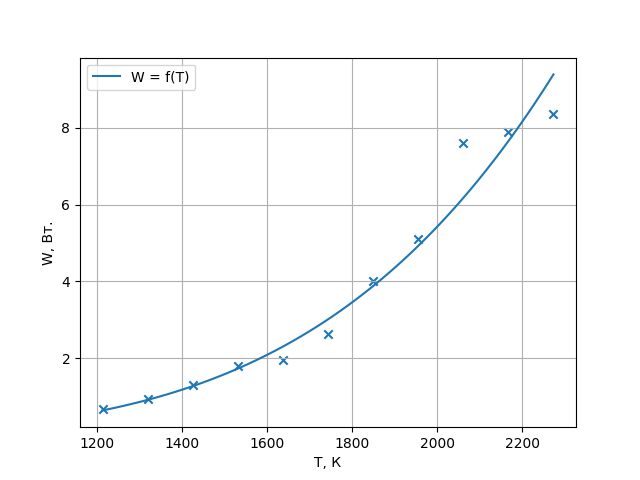
\includegraphics{regular_plot.png}
    \centering
    \caption{График $W = f(T)$}
    \label{pic:W}
\end{figure}

\begin{figure}[H]
    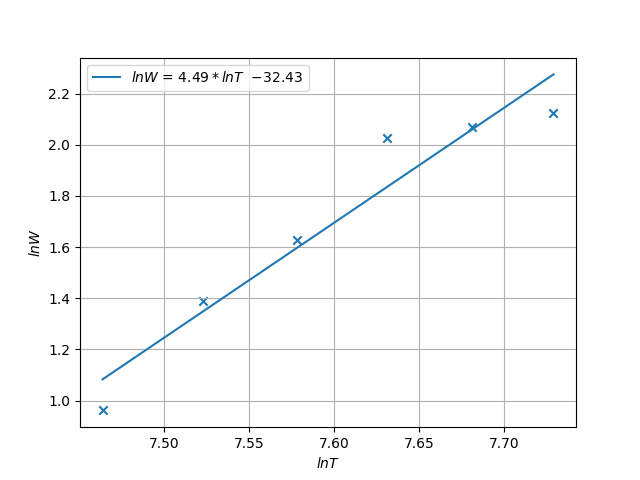
\includegraphics{log_plot.png}
    \centering
    \caption{График $\ln W = f(\ln T)$}
    \label{pic:lnW}
\end{figure}


\point Из графика с помощью МНК получаем:

\begin{align*}
    n &= 4.49 \pm 0.12 \\
    \ln (\varepsilon_T \sigma S) &= -32.43 \pm 0.01
\end{align*}

Стоит отметить, что график строился только по для точек, у которых $T > 1700~K$. Это сделано из-за того, что при меньших температурах существует зависимость $S(T)$, которую невозможно учесть. Начиная же с таких температур нить накаляется полностью, т.~е. $S = 0.36~см^2 = const$. Но при этом необходимо учесть, что $\varepsilon_T$ тоже зависит от температуры. Для этого была использована таблица \ref{tab:epsT}.

Теоретическое значение $n = 4$ \eqref{eq:s-b}. То етсь, полученное экспериментальное значение с хорошей точностью сходится с теоретическим.


\point Для каждого значения $T > 1700~K$ найдём постоянную Стефана-Больцмана и постоянную Планка по формулам \eqref{eq:s-b} и  \eqref{eq:h-sigma}. Результаты представлены в таблицах \ref{tab:sigma} и \ref{tab:h}.

\begin{table}[H]
    \centering
    \begin{tabular}{|c|c|c|c|c|c|c|}
        \hline
        $T~K$,   &  1743	 & 1849	 & 1955	 & 2061	 & 2167	 & 2273	\\ \hline

        $\sigma, \dfrac{Вт}{см^2 \cdot К^4}$ & $3.70 \cdot 10^{-12}$	 & $4.18 \cdot 10^{-12}$	 & $3.99 \cdot 10^{-12}$	 & $4.53 \cdot 10^{-12}$	 & $3.65 \cdot 10^{-12}$	 & $3.03 \cdot 10^{-12}$	 \\ \hline
    \end{tabular}
    \caption {$\sigma (T)$}
    \label{tab:sigma}
\end{table}


\begin{table}[H]
    \centering
    \begin{tabular}{|c|c|c|c|c|c|c|}
        \hline
        $T~K$,   &  1743	 & 1849	 & 1955	 & 2061	 & 2167	 & 2273	\\ \hline
        $h, Дж \cdot с$ & $7.64 \cdot 10^{-34}$	 & $7.33 \cdot 10^{-34}$	 & $7.45 \cdot 10^{-34}$	 & $7.14 \cdot 10^{-34}$	 & $7.67 \cdot 10^{-34}$	 & $8.17 \cdot 10^{-34}$	\\ \hline
    \end{tabular}
    \caption {$h (T)$}
    \label{tab:h}
\end{table}

\parag {Заключение} ~\\
В ходе лабораторной работы при помощи модели абсолютно чёрного тела были проведены измерения температуры, определены постоянные Планка и Стефана-Больцмана. Некоторые из результатов совпали с теоретическими, некоторые -- нет. Последне может быть связано с неверно указанной эффективной площадью проволоки. 

\end{document}
